\documentclass[12pt]{article}

\usepackage{fancyhdr}
\usepackage{amsthm}
\usepackage{amsmath}
\usepackage{graphicx}
\usepackage{amssymb}
\usepackage{esint}
\usepackage{subfigure}
\usepackage{color}
\usepackage{moreverb}
\usepackage{wrapfig}
\usepackage{subfig}
\usepackage{changepage}


\textwidth 17cm \topmargin -1cm \oddsidemargin 0cm \textheight 21.5cm
\pagestyle{empty} \pagestyle{fancyplain}
\lhead[\fancyplain{}{}]{\fancyplain{}{{\sc Myles Adams}}}
\chead[\fancyplain{}{}]{\fancyplain{}{{\sc CS 111 Final}}}
\rhead[\fancyplain{}{}]{\fancyplain{}{{\sc Fall 2017}}}

\newcommand{\etal}{\textit{et al. }}

\begin{document}
\centerline{\Large\textbf{CS 111 Final}}
\vspace{.5cm}

\section*{Problem 1}\label{sec::Problem1}
\subsection*{Introduction}
The goal of this first problem is to find the optimal time it takes to boil a potato. In order to do this, we will approximate the shape of a potato as a two dimensional 4cm by 5cm rectangle. At time $t_{start}=0$ a pan is filled with water and contains the potato; it is placed on the stove top. The initial temperature of the potato and water is $T_{room} = 20^\circ C$. The water temperature then quickly rises from $20^\circ c$ to $100^\circ C$ in 60 seconds and then stays at $100^\circ C$. This is modeled by the equation $T_{water} = min(20 + 80\frac{t}{60}, 100)$. Due to the thermal conduction heat propagates from water inside the potato. At the temperature of $T_{cooking} = 65^\circ C$, the cellular structure of the potato begins to change and the starch starts to gelatinize. We will assume that it takes 5 minutes (300 seconds) for the potato to fully cook once the temperature of the potato has reached the temperature $T_{cooking}$.

The temperature T = T(t,x,y) inside the potato satisfies the heat equation (diffusion equation) shown below:
\begin{center}
$\frac{\partial T}{\partial t}= \lambda \Delta T ,\hspace{.3cm}(x,y) \in \Omega$
\end{center}
with the boundary conditions:
\begin{center}
$T(t,x,y) = T_{water}(t),\hspace{.3cm}(x,y) \in \partial \Omega$
\end{center}
and the initial conditions:
\begin{center}
$T(0,x,y) = T_{room}(t),\hspace{.3cm}(x,y) \in \partial \Omega$
\end{center}
where $\lambda$ is the thermal diffusivity constant of the potato's material. $\Omega$ and $\partial \Omega$ denote both the domain occupied in space by the potato and the boundary of this domain.

\subsection*{Part A}
\subsection*{Part B}
\begin{table}[]
\centering
\label{p1_table}
\begin{tabular}{|l|l|l|ll}
\cline{1-3}
Resolution & Error       & Order of Accuracy &  &  \\ \cline{1-3}
25 x 30    & 0.000583961 & 0                 &  &  \\ \cline{1-3}
50 x 60    & 0.000278453 & 1.06844           &  &  \\ \cline{1-3}
100 x 120  & 0.000136207 & 1.03163           &  &  \\ \cline{1-3}
\end{tabular}
\end{table}
\subsection*{Part C}

\begin{figure}[htb]%
    \centering
    {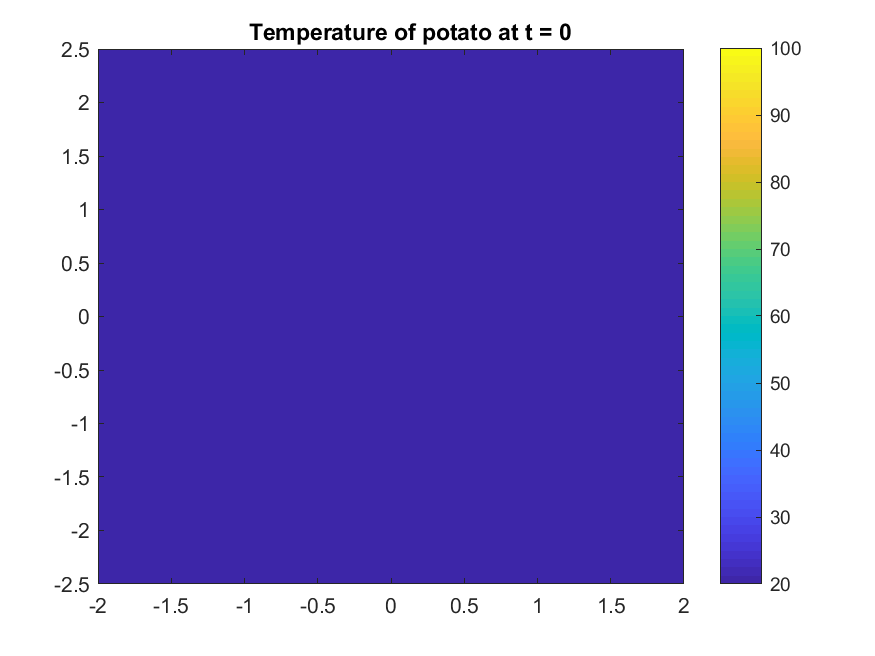
\includegraphics[width=8cm]{Problem1_fig1.png}}%
    \qquad
    {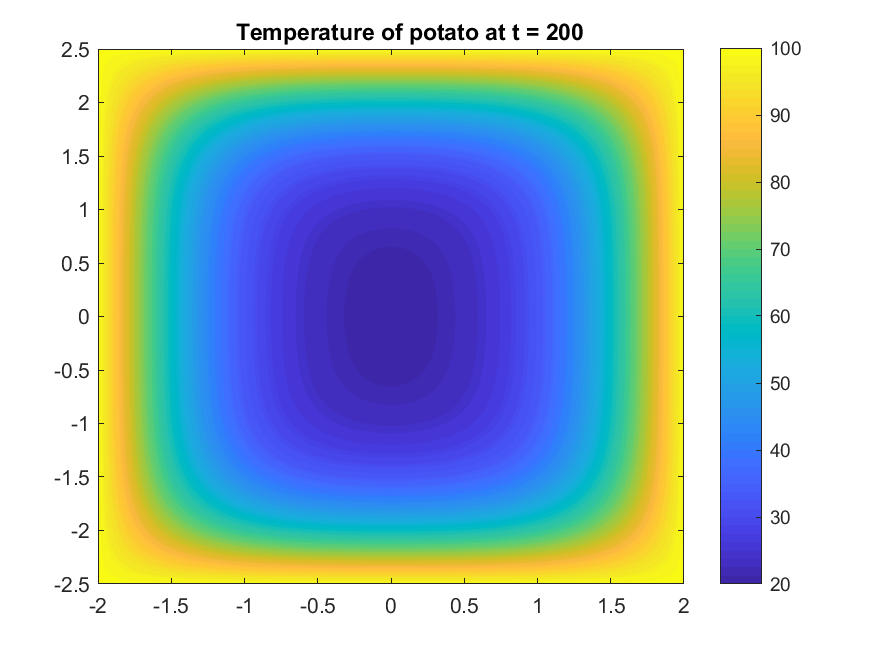
\includegraphics[width=8cm]{Problem1_fig2.png}}%
    \label{fig:p1_fig1-2}%
\end{figure}

\begin{figure}[htb]%
    \centering
    {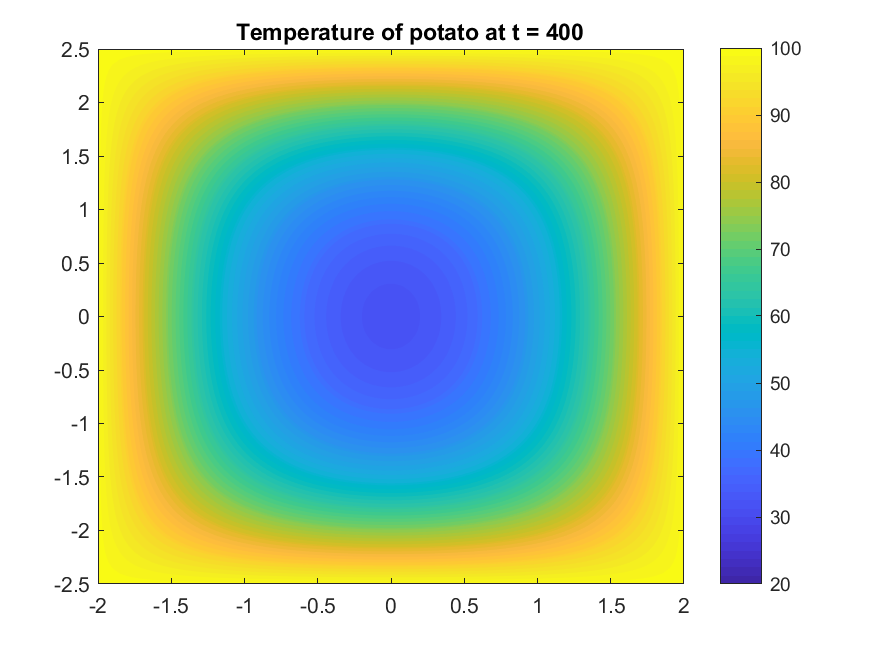
\includegraphics[width=8cm]{Problem1_fig3.png}}%
    \qquad
    {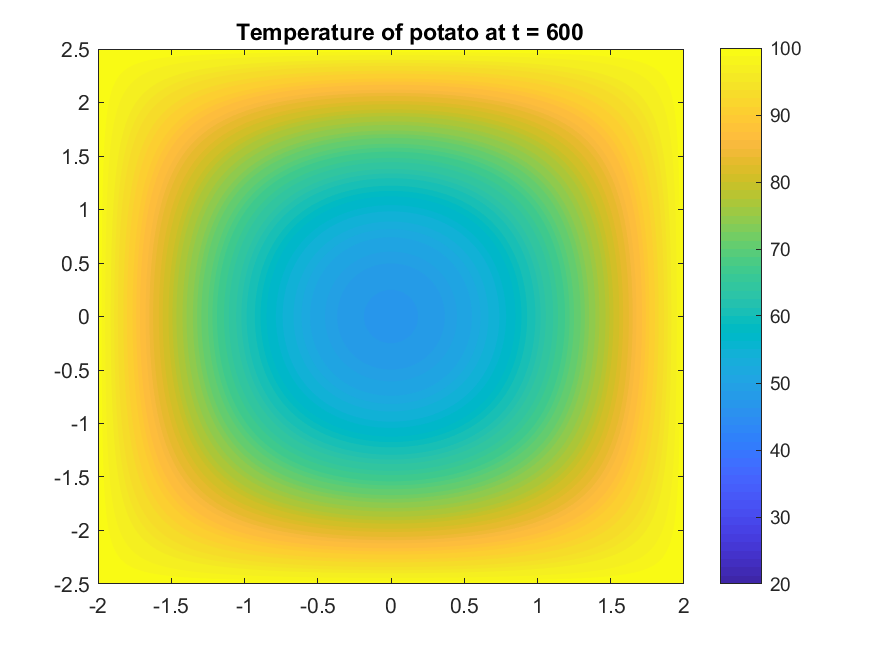
\includegraphics[width=8cm]{Problem1_fig4.png}}%
    \label{fig:p1_fig3-4}%
    \caption*{Temperature ($^{\circ}$C) throughout the potato at various times}
\end{figure}

\begin{figure}[htb]
\centering
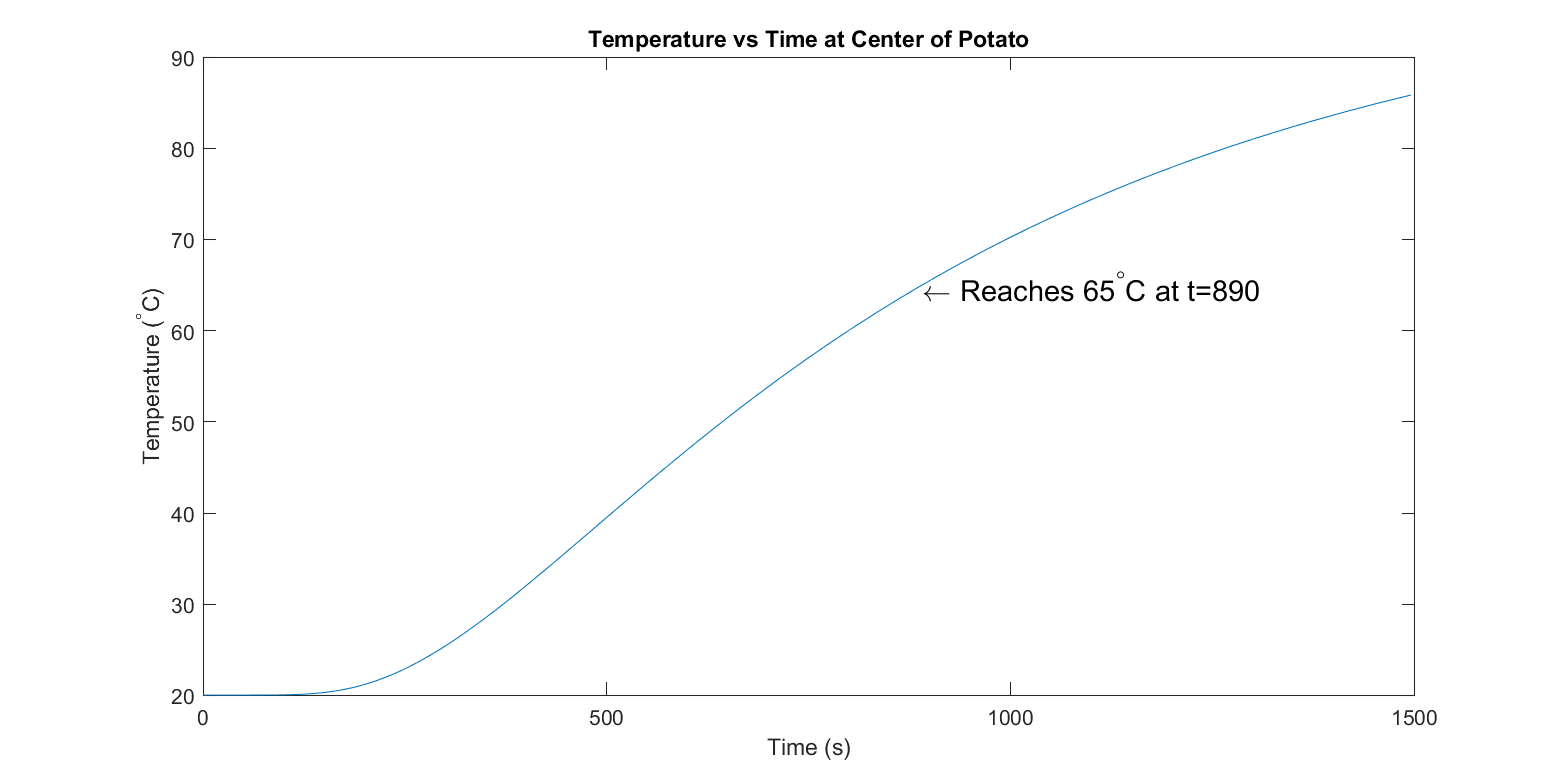
\includegraphics[width=1\textwidth]{Problem1_fig5.png}
\caption*{Temperature ($^{\circ}$C) at the center of potato vs time}
\label{fig::p1_fig5}
\end{figure}

\section*{Problem 2}\label{sec::Problem2}
\subsection*{Introduction}
\subsection*{Part A}
\subsection*{Part B}
\begin{table}[]
\centering
\label{p2_table}
\begin{tabular}{|l|l|l|}
\hline
Resolution & Error      & Order of Accuracy \\ \hline
20 x 15    & 0.0240409  & 0                 \\ \hline
40 x 30    & 0.0119852  & 1.00424           \\ \hline
80 x 60    & 0.00598461 & 1.00193           \\ \hline
160 x 120  & 0.00299154 & 1.00037           \\ \hline
\end{tabular}
\end{table}
\subsection*{Part C}
\begin{figure}[htp]
\begin{adjustwidth}{-2cm}{-2cm}
\centering
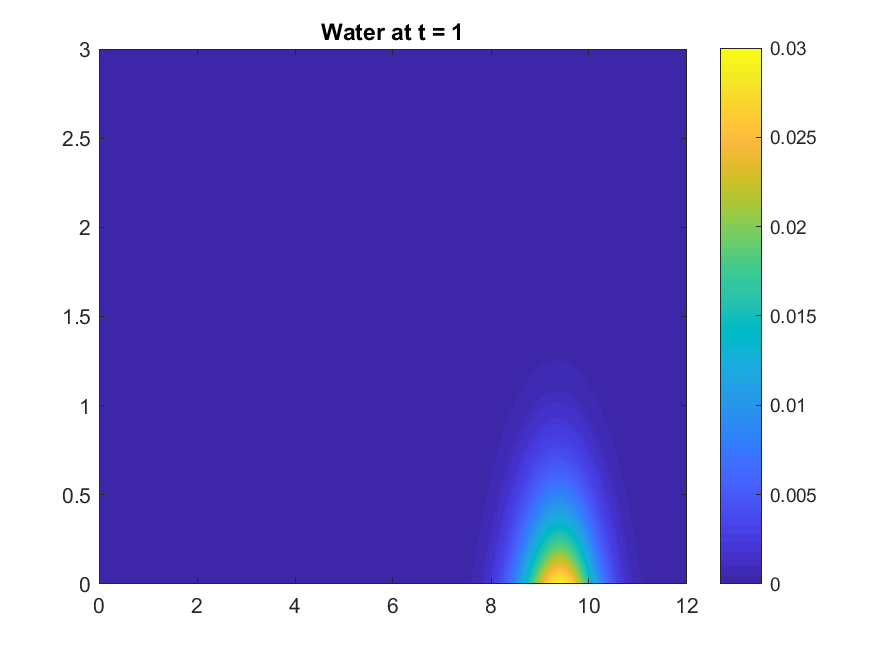
\includegraphics[width=.41\textwidth]{Problem2_fig1.png}\hfill
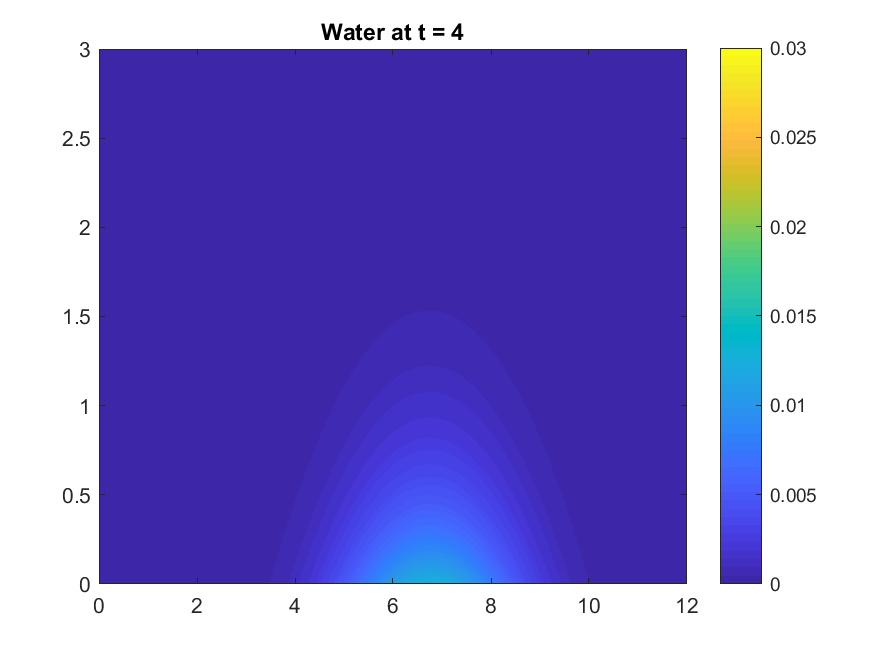
\includegraphics[width=.41\textwidth]{Problem2_fig2.png}\hfill
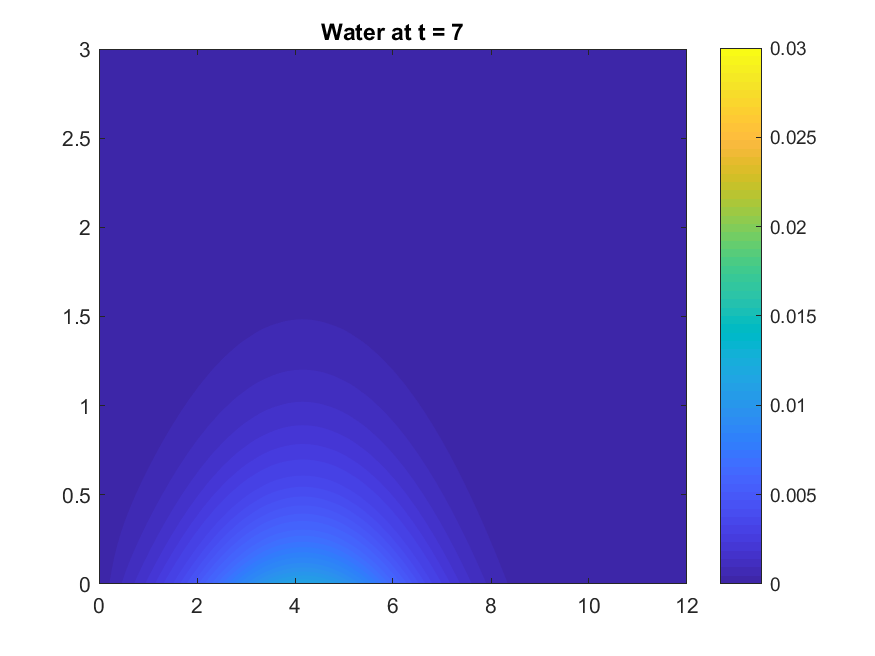
\includegraphics[width=.41\textwidth]{Problem2_fig3.png}
\label{fig:p2_fig1-3}
\end{adjustwidth}
\end{figure}

\begin{figure}[htb]
\begin{adjustwidth}{-2cm}{-2cm}
\centering
\hspace{-.9cm}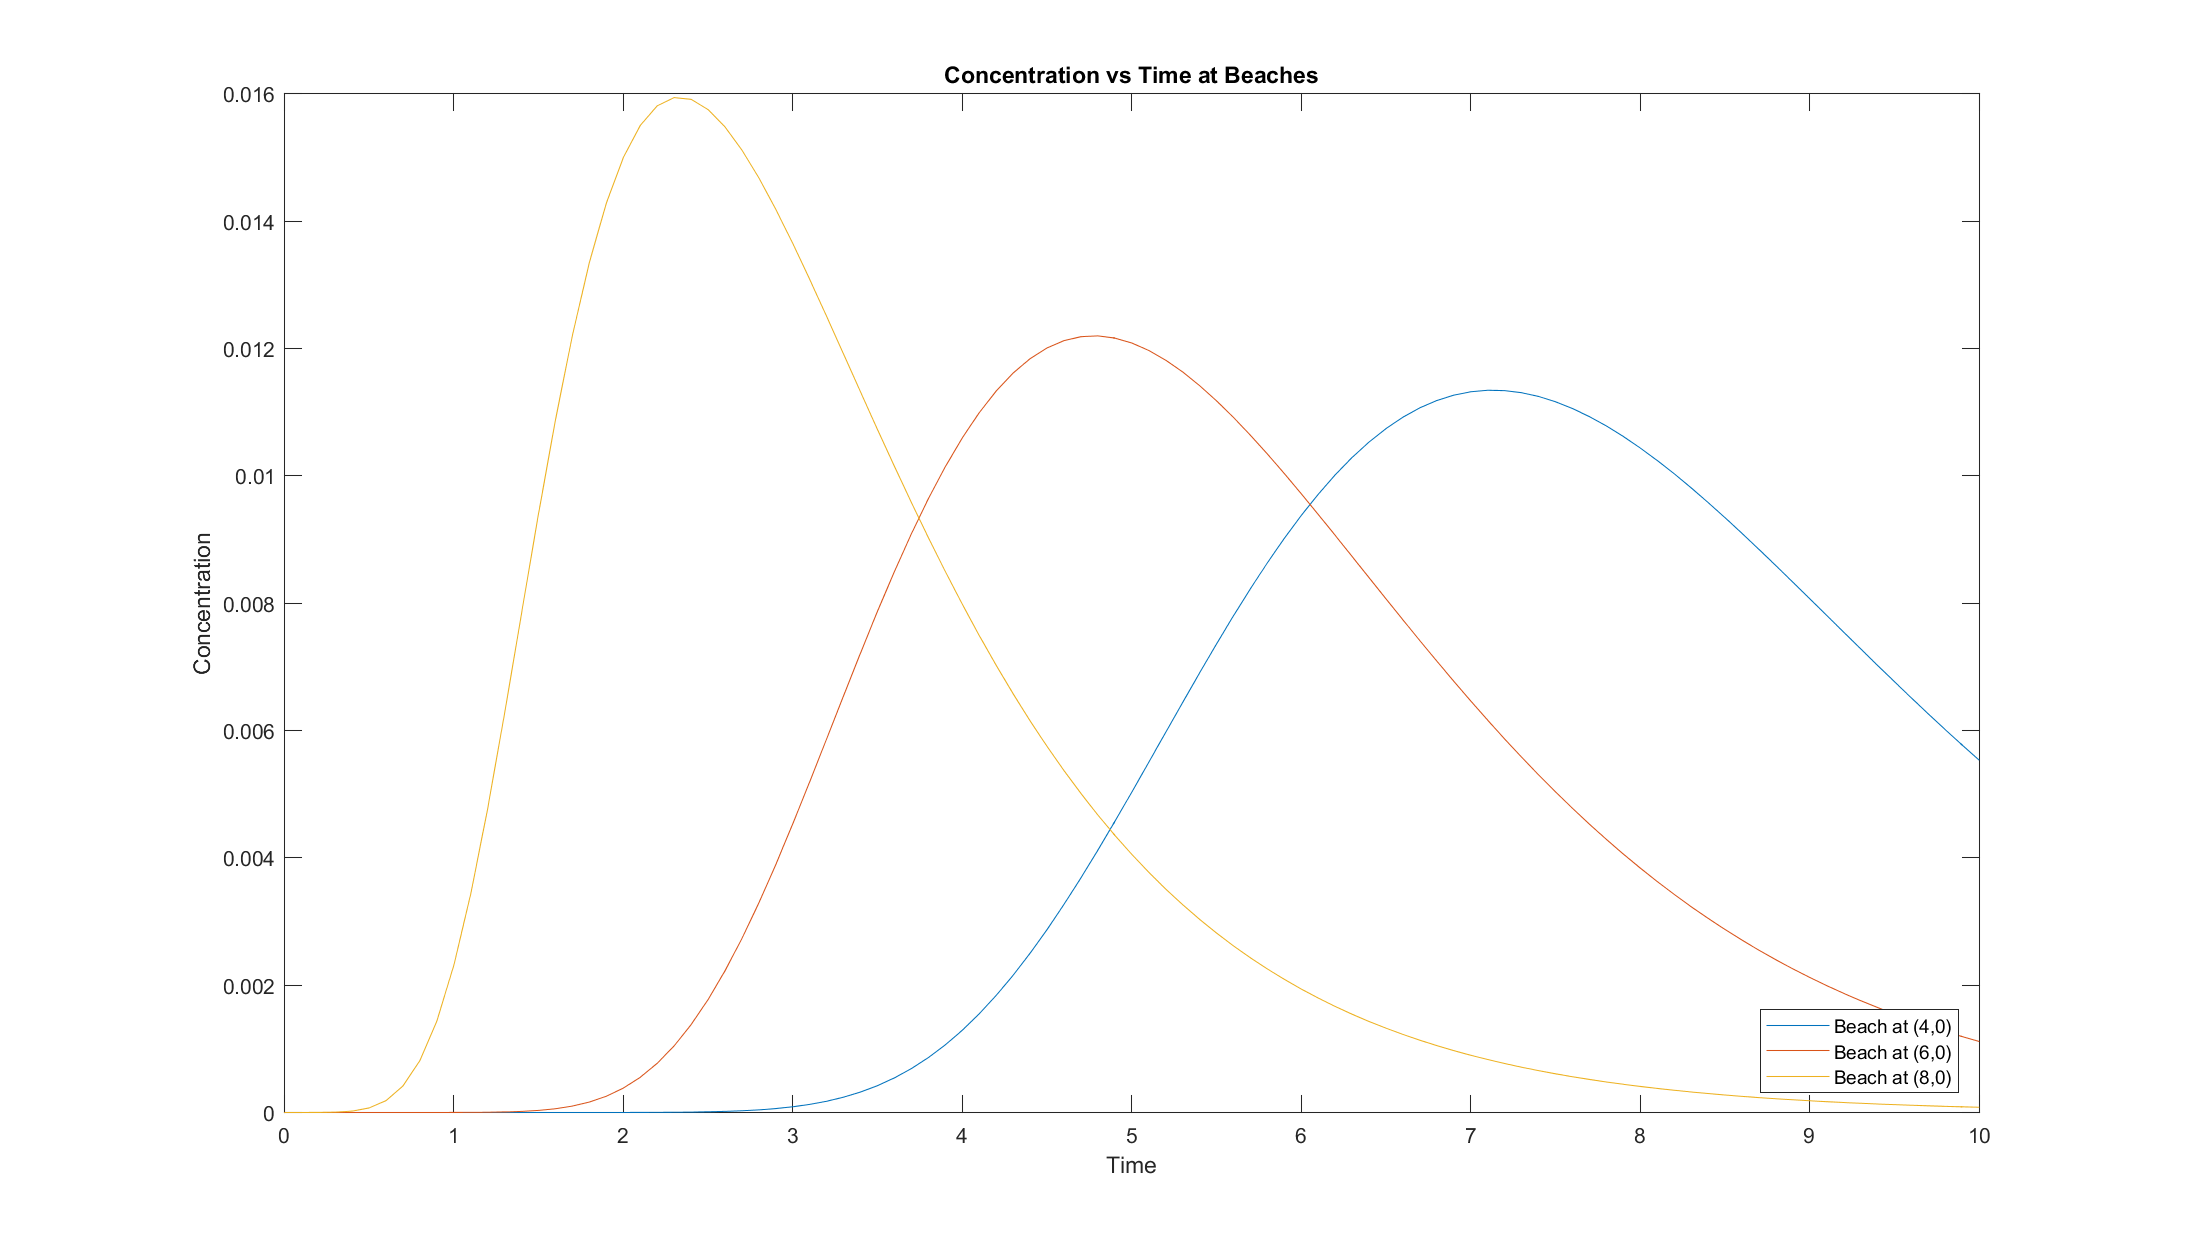
\includegraphics[width=1.2\textwidth]{Problem2_fig4.png}
\caption*{Concentration of oil at each beach vs time}
\label{fig::p2_fig5}
\end{adjustwidth}
\end{figure}


\newpage
\clearpage
\setcounter{page}{1} \pagestyle{empty}
\section*{References}\label{sec::References}
\begin{itemize}
\item [1] Daniil Bochkov, CS 111 - Introduction to Computational Science - Midterm, Fall 2017
\item [2] Daniil Bochkov, CS 111 - Introduction to Computational Science - Lecture 4 - High-Order Methods, Fall 2017
\item [3] Daniil Bochkov, CS 111 - Introduction to Computational Science - Lecture 6 - Systems of ODEs,  Fall 2017
\item [4] Daniil Bochkov, CS 111 - Introduction to Computational Science - Lecture 7 - High-Order ODEs, Fall 2017
\end{itemize}
\end{document}
